\documentclass[
  jou,
  floatsintext,
  longtable,
  nolmodern,
  notxfonts,
  notimes,
  12pt,
  colorlinks=true,linkcolor=blue,citecolor=blue,urlcolor=blue]{apa7}

\usepackage{amsmath}
\usepackage{amssymb}
\usepackage{setspace}


\usepackage[bidi=default]{babel}
\babelprovide[main,import]{english}


% get rid of language-specific shorthands (see #6817):
\let\LanguageShortHands\languageshorthands
\def\languageshorthands#1{}

\RequirePackage{longtable}
\RequirePackage{threeparttablex}

\usepackage{framed}


\makeatletter
\renewcommand{\paragraph}{\@startsection{paragraph}{4}{\parindent}%
	{0\baselineskip \@plus 0.2ex \@minus 0.2ex}%
	{-.5em}%
	{\normalfont\normalsize\bfseries\typesectitle}}

\renewcommand{\subparagraph}[1]{\@startsection{subparagraph}{5}{0.5em}%
	{0\baselineskip \@plus 0.2ex \@minus 0.2ex}%
	{-\z@\relax}%
	{\normalfont\normalsize\bfseries\itshape\hspace{\parindent}{#1}\textit{\addperi}}{\relax}}
\makeatother




% longtable is already loaded via doc-class.tex (apa7 class option) and
% apatemplate.tex (\RequirePackage{longtable}). Keep booktabs here so raw
% LaTeX tables using \toprule/\midrule still render even without Pandoc table
% nodes.
\usepackage{booktabs, multirow, multicol, colortbl, hhline, caption, array, float, xpatch}
\usepackage{subcaption}


\renewcommand\thesubfigure{\Alph{subfigure}}
\setcounter{topnumber}{2}
\setcounter{bottomnumber}{2}
\setcounter{totalnumber}{4}
\renewcommand{\topfraction}{0.85}
\renewcommand{\bottomfraction}{0.85}
\renewcommand{\textfraction}{0.15}
\renewcommand{\floatpagefraction}{0.7}

\usepackage{tcolorbox}
\tcbuselibrary{listings,theorems, breakable, skins}
\usepackage{fontawesome5}

\definecolor{quarto-callout-color}{HTML}{909090}
\definecolor{quarto-callout-note-color}{HTML}{0758E5}
\definecolor{quarto-callout-important-color}{HTML}{CC1914}
\definecolor{quarto-callout-warning-color}{HTML}{EB9113}
\definecolor{quarto-callout-tip-color}{HTML}{00A047}
\definecolor{quarto-callout-caution-color}{HTML}{FC5300}
\definecolor{quarto-callout-color-frame}{HTML}{ACACAC}
\definecolor{quarto-callout-note-color-frame}{HTML}{4582EC}
\definecolor{quarto-callout-important-color-frame}{HTML}{D9534F}
\definecolor{quarto-callout-warning-color-frame}{HTML}{F0AD4E}
\definecolor{quarto-callout-tip-color-frame}{HTML}{02B875}
\definecolor{quarto-callout-caution-color-frame}{HTML}{FD7E14}

%\newlength\Oldarrayrulewidth
%\newlength\Oldtabcolsep


\usepackage{hyperref}
\usepackage[protrusion=true]{microtype}


\providecommand{\tightlist}{%
  \setlength{\itemsep}{0pt}\setlength{\parskip}{0pt}}
\usepackage{longtable,booktabs,array}
\usepackage{calc} % for calculating minipage widths
% Correct order of tables after \paragraph or \subparagraph
\usepackage{etoolbox}
\makeatletter
\patchcmd\longtable{\par}{\if@noskipsec\mbox{}\fi\par}{}{}
\makeatother
% Allow footnotes in longtable head/foot
\IfFileExists{footnotehyper.sty}{\usepackage{footnotehyper}}{\usepackage{footnote}}
\makesavenoteenv{longtable}

\usepackage{graphicx}
\makeatletter
\newsavebox\pandoc@box
\newcommand*\pandocbounded[1]{% scales image to fit in text height/width
  \sbox\pandoc@box{#1}%
  \Gscale@div\@tempa{\textheight}{\dimexpr\ht\pandoc@box+\dp\pandoc@box\relax}%
  \Gscale@div\@tempb{\linewidth}{\wd\pandoc@box}%
  \ifdim\@tempb\p@<\@tempa\p@\let\@tempa\@tempb\fi% select the smaller of both
  \ifdim\@tempa\p@<\p@\scalebox{\@tempa}{\usebox\pandoc@box}%
  \else\usebox{\pandoc@box}%
  \fi%
}
% Set default figure placement to htbp
\def\fps@figure{htbp}
\makeatother


% definitions for citeproc citations
\NewDocumentCommand\citeproctext{}{}
\NewDocumentCommand\citeproc{mm}{%
  \begingroup\def\citeproctext{#2}\cite{#1}\endgroup}
\makeatletter
 % allow citations to break across lines
 \let\@cite@ofmt\@firstofone
 % avoid brackets around text for \cite:
 \def\@biblabel#1{}
 \def\@cite#1#2{{#1\if@tempswa , #2\fi}}
\makeatother
\newlength{\cslhangindent}
\setlength{\cslhangindent}{1.5em}
\newlength{\csllabelwidth}
\setlength{\csllabelwidth}{3em}
\newenvironment{CSLReferences}[2] % #1 hanging-indent, #2 entry-spacing
 {\begin{list}{}{%
  \setlength{\itemindent}{0pt}
  \setlength{\leftmargin}{0pt}
  \setlength{\parsep}{0pt}
  % turn on hanging indent if param 1 is 1
  \ifodd #1
   \setlength{\leftmargin}{\cslhangindent}
   \setlength{\itemindent}{-1\cslhangindent}
  \fi
  % set entry spacing
  \setlength{\itemsep}{#2\baselineskip}}}
 {\end{list}}
\usepackage{calc}
\newcommand{\CSLBlock}[1]{\hfill\break\parbox[t]{\linewidth}{\strut\ignorespaces#1\strut}}
\newcommand{\CSLLeftMargin}[1]{\parbox[t]{\csllabelwidth}{\strut#1\strut}}
\newcommand{\CSLRightInline}[1]{\parbox[t]{\linewidth - \csllabelwidth}{\strut#1\strut}}
\newcommand{\CSLIndent}[1]{\hspace{\cslhangindent}#1}





\usepackage{newtx}

\defaultfontfeatures{Scale=MatchLowercase}
\defaultfontfeatures[\rmfamily]{Ligatures=TeX,Scale=1}





\title{Towards an Active Inference Personality Framework: The Core
Priors Cascade Model of the Self}


\shorttitle{Core Priors Cascade Model}


\usepackage{etoolbox}






\author{Dominique Makowski}



\authorsaffiliations{
{School of Psychology, University of Sussex},{Sussex Centre for
Consciousness Science, University of Sussex}}




\leftheader{Makowski}



\abstract{The Core Priors Cascade (CPC) Model is a hierarchical
generative account of personality and individual differences grounded in
the Free Energy Principle and active inference. In contrast to
descriptive psychometric frameworks that identify behavioural
phenotypes, the CPC Model proposes that observable personality traits
represent the downstream expressions of deeply entrenched probabilistic
parameters: hierarchically organised expectations and precision
settings. These govern an agent's structural expectations and
information processing biases. These hyper-priors are organised into
three groups: Existential Expectations, encoding global parameters of
volatility, agency, and temporal self-extension; Boundary and Relational
Biases, governing Markov blanket permeability and sensory grounding; and
Operational Expectations and Biases, regulating error-resolution
strategies and self-model coherence. From this hierarchical structure,
five latent factors are hypothesised. These factors (Epistemic
Plasticity, Cybernetic Stability, Blanket Permeability, Temporal
Extension, and Self-Model Stability) are argued to constitute the
generative mechanisms underlying the phenotypic variance captured by
existing descriptive models including the Big Five, behavioural
inhibition and activation systems, attachment theory, and sensation
seeking. The CPC Model is presented as a principled, mechanistic
complement to existing descriptive frameworks, offering testable
predictions regarding the hierarchical structure of individual
differences and differential psychopathological
vulnerability.  \section{Impact Statement} \noindent The Core Priors
Cascade Model provides a mechanistic, mathematically grounded account of
how hierarchical expectations and precision biases generate the full
range of observable personality phenotypes, offering a principled bridge
between the Free Energy Principle and the scientific study of individual
differences. }

\keywords{active inference, free energy
principle, personality, individual differences, predictive
processing, cybernetics, expectations, precision bias}

\authornote{\par{\addORCIDlink{Dominique
Makowski}{0000-0001-5375-9967}} 
\par{ }
\par{   The authors have no conflicts of interest to disclose.    Author
roles were classified using the Contributor Role Taxonomy (CRediT;
\href{https://credit.niso.org}{credit.niso.org}) as follows:  Dominique
Makowski:   Project administration, Data curation, Formal
Analysis, Investigation, Visualization, Writing -- original
draft, Writing -- review \& editing}
\par{Correspondence concerning this article should be addressed
to Dominique
Makowski, Email: \href{mailto:D.Makowski@sussex.ac.uk}{D.Makowski@sussex.ac.uk}}
}

\usepackage{pbalance}
% \usepackage{float}
\makeatletter
\let\oldtpt\ThreePartTable
\let\endoldtpt\endThreePartTable
\def\ThreePartTable{\@ifnextchar[\ThreePartTable@i \ThreePartTable@ii}
\def\ThreePartTable@i[#1]{\begin{figure}[!htbp]
\onecolumn
\begin{minipage}{0.485\textwidth}
\oldtpt[#1]
}
\def\ThreePartTable@ii{\begin{figure}[!htbp]
\onecolumn
\begin{minipage}{0.48\textwidth}
\oldtpt
}
\def\endThreePartTable{
\endoldtpt
\end{minipage}
\twocolumn
\end{figure}}
\makeatother


\makeatletter
\let\endoldlt\endlongtable		
\def\endlongtable{
\hline
\endoldlt}
\makeatother

\newenvironment{twocolumntable}% environment name
{% begin code
\begin{table*}[!htbp]%
\onecolumn%
}%
{%
\twocolumn%
\end{table*}%
}% end code

\urlstyle{same}



\makeatletter
\@ifpackageloaded{caption}{}{\usepackage{caption}}
\AtBeginDocument{%
\ifdefined\contentsname
  \renewcommand*\contentsname{Table of contents}
\else
  \newcommand\contentsname{Table of contents}
\fi
\ifdefined\listfigurename
  \renewcommand*\listfigurename{List of Figures}
\else
  \newcommand\listfigurename{List of Figures}
\fi
\ifdefined\listtablename
  \renewcommand*\listtablename{List of Tables}
\else
  \newcommand\listtablename{List of Tables}
\fi
\ifdefined\figurename
  \renewcommand*\figurename{Figure}
\else
  \newcommand\figurename{Figure}
\fi
\ifdefined\tablename
  \renewcommand*\tablename{Table}
\else
  \newcommand\tablename{Table}
\fi
}
\@ifpackageloaded{float}{}{\usepackage{float}}
\floatstyle{ruled}
\@ifundefined{c@chapter}{\newfloat{codelisting}{h}{lop}}{\newfloat{codelisting}{h}{lop}[chapter]}
\floatname{codelisting}{Listing}
\newcommand*\listoflistings{\listof{codelisting}{List of Listings}}
\makeatother
\makeatletter
\makeatother
\makeatletter
\@ifpackageloaded{caption}{}{\usepackage{caption}}
\@ifpackageloaded{subcaption}{}{\usepackage{subcaption}}
\makeatother

% From https://tex.stackexchange.com/a/645996/211326
%%% apa7 doesn't want to add appendix section titles in the toc
%%% let's make it do it
\makeatletter
\xpatchcmd{\appendix}
  {\par}
  {\addcontentsline{toc}{section}{\@currentlabelname}\par}
  {}{}
\makeatother

%% Disable longtable counter
%% https://tex.stackexchange.com/a/248395/211326

\usepackage{etoolbox}

\makeatletter
\patchcmd{\LT@caption}
  {\bgroup}
  {\bgroup\global\LTpatch@captiontrue}
  {}{}
\patchcmd{\longtable}
  {\par}
  {\par\global\LTpatch@captionfalse}
  {}{}
\apptocmd{\endlongtable}
  {\ifLTpatch@caption\else\addtocounter{table}{-1}\fi}
  {}{}
\newif\ifLTpatch@caption
\makeatother

\begin{document}

\maketitle




\setlength\LTleft{0pt}



\ifdefined\Shaded\renewenvironment{Shaded}{\begin{snugshade}\begin{singlespace}}{\end{singlespace}\end{snugshade}}\fi


Personality psychology faces a persistent explanatory gap. While
descriptive frameworks, such as the Big Five model of personality traits
(\citeproc{ref-goldberg1990alternative}{Goldberg, 1990};
\citeproc{ref-mccrae1992introduction}{McCrae \& John, 1992}), have
proven remarkably successful at organising individual differences in
behaviour, affect, and cognition, their structural parsimony comes at a
theoretical cost. These models describe what varies across individuals
but offer limited purchase on why such variation exists or how it is
generated and maintained. Comprehensive mechanistic accounts capable of
specifying the processes that produce the characteristic patterns we
label as Neuroticism, Openness, or Conscientiousness are relatively
scarce.

Several generative frameworks have attempted to bridge this
descriptive-process divide. The Cognitive-Affective Personality System
(CAPS, \citeproc{ref-mischel1995cognitive}{Mischel \& Shoda, 1995})
conceptualises personality as a network of interacting cognitive and
affective units, while Whole Trait Theory
(\citeproc{ref-fleeson2015whole}{Fleeson \& Jayawickreme, 2015}) frames
traits as density distributions of momentary states. More recently,
Cybernetic Big Five Theory (CB5T,
\citeproc{ref-deyoung2015cybernetic}{DeYoung, 2015}) has offered a
functionalist account of traits as parameters of a cybernetic system
optimising for distinct goals. Yet, while these models successfully
introduce process dynamics, they largely lack a unified mathematical
ontology to explain why certain cognitive-affective parameters reliably
coalesce into the stable phenotypic attractors we observe.

The Free Energy Principle (FEP, \citeproc{ref-friston2010free}{Friston,
2010}) and its process theory, active inference, offer a principled
candidate for such a generative account. Under the FEP, all
self-organising biological systems minimise the upper bound on their own
surprise, formally defined as variational free energy, by maintaining
and continuously updating probabilistic generative models of their
sensory environment. This minimisation operates through two
complementary pathways: perceptual inference (revising internal models
to fit sensory signals) and active inference (acting on the world to
bring sensory signals into conformity with predictions).

Applied to the domain of personality, this framework implies that
characteristic individual differences do not reflect fixed trait
properties of the organism but rather the downstream consequences of
deeply entrenched probabilistic parameters. To ground these parameters
in the formal mathematics of the FEP, the framework explicitly
distinguishes between \emph{expectations} (the locations or means of an
internal distribution, \(\mu\)) and \emph{biases} (the precisions,
gains, or relative inverse-variance ratios assigned to different
processing channels, \(\pi\)). What are colloquially called ``prior
preferences'' or ``drives'' are recast under this architecture as state
expectations equipped with exceptionally high precision constraints.
These foundational parameters scaffold the agent's predictive
architecture and act as strong constraints on all subsequent inference
and action.

The present paper proposes the Core Priors Cascade (CPC) Model of
Personality, a hierarchical framework that defines and organises these
foundational expectations and biases across levels of abstraction and
influence. At the apex sit \emph{Existential Expectations}, representing
the most fundamental assumptions the agent holds about the volatility of
its environment, the tractability of prediction error through action,
and the ultimate temporal horizon of the self. These global location
parameters cascade downward to constrain a second group of
\emph{Boundary and Relational Biases}. This category governs the
precision weighting, permeability, and sensory grounding of the agent's
Markov blanket, the statistical boundary demarcating self from
environment (\citeproc{ref-friston2019markov}{Friston, 2019}). These in
turn constrain a third level of \emph{Operational Expectations and
Biases}, which dictate the agent's characteristic strategies for
minimizing free energy across the perception-action cycle.

The CPC Model is explicitly positioned not as a replacement for existing
descriptive frameworks but as a generative account of the mechanisms
underlying the phenotypes those frameworks identify. The Big Five
describe individual differences at the level of behavioural output, and
the Cybernetic Big Five Theory begins to explain them at the level of
cybernetic function. The CPC Model proposes to account for both at the
level of the hierarchical expectation and precision structure from which
such function emerges. It thereby offers testable structural predictions
and a principled basis for understanding individual differences in
general temperament as well as psychopathological vulnerability.

\section{The Core Priors Cascade
Model}\label{the-core-priors-cascade-model}

The central architectural claim of the CPC Model is that the cascade is
not merely correlational. Higher-level parameters do not just co-vary
with lower-level ones; they constrain the solution space available to
them. An existential-level configuration of extreme expected volatility
and low expected tractability forecloses certain operational-level
strategies. This hierarchical determination is what differentiates the
CPC Model from multivariate trait models in which dimensions are
statistically correlated but conceptually orthogonal.

A productive conceptual frame for this cascade architecture is that of a
\emph{free energy landscape}. This is a topographic surface on which the
agent's achievable parameter configurations are mapped against their
associated expected free energy. Stable personality configurations
correspond to local minima acting as \emph{attractor basins} into which
the system settles and from which it resists displacement.

The binary distinction between expectations and biases clarifies this
topology: - \textbf{Expectations (Locations)} determine \emph{where} the
attractor basins are carved into the landscape---the specific states and
environmental regularities the agent assumes to be true. -
\textbf{Biases (Precisions)} determine \emph{how deep and steep} those
basins are, defining the rigid boundaries of the walls and dictating how
easily the system can be bumped out of its habitual states by sensory
noise.

Deeply entrenched existential expectations carve deep attractors with
steep precision walls that demand substantial perturbation to escape.
Mild challenges to the generative model produce only local oscillations
within the basin. However, more substantial perturbations, such as
developmental transitions, significant relational experiences, or
sustained therapeutic intervention, may shift the system to an adjacent
attractor. Catastrophic destabilisation may temporarily flatten the
landscape entirely, transiently liberating the system from habitual
precision constraints.

The \emph{valleys} of this landscape are the expectations themselves.
Characteristic personality configurations represent the stable dynamical
states of an agent's free energy landscape. Psychopathological
trajectories can be understood as transitions between basins, as
trapping within anomalously deep basins, or as the fragmentation of a
landscape too shallow to sustain coherent stable states. This framing
also accommodates the bidirectional dynamics of the cascade. While
higher-level parameters constrain the solution space for lower-level
configurations, bottom-up neuroplasticity continuously reshapes the
landscape through experience and development, gradually deepening or
shallowing the attractor basins themselves.

The landscape also has an overall topology that shapes all local
dynamics. Death, defined as systemic cessation or the dissolution of the
agent's self-organising boundary, is not merely one attractor basin
among many but the global minimum. It is the deepest point toward which
any finite system will eventually tend. All other personality
configurations are metastable states on a landscape that tilts, over
sufficiently long timescales, toward this terminus. The terminal
expectation, described below, governs how consciously and at what
distance the agent orients to this underlying structure.

The following sections specify the dimensions at each level, moving from
the most global and abstract to the most proximal and context-sensitive.

\subsection{Existential Hyperpriors}\label{existential-hyperpriors}

Existential expectations occupy the apex of the cascade hierarchy. They
encode the agent's most fundamental assumptions about the nature of its
environment and the ultimate tractability of its predictive project.
Because they operate as location parameters (\(\mu\)) at the highest
level of abstraction, perturbations at this level propagate throughout
the entire system. They are described here as ``existential'' because
they concern not merely strategic preferences for error minimisation but
the agent's basic orientation to its own existence in time, addressing
questions of agency, safety, and finitude.

\subsubsection{Volatility Expectation}\label{volatility-expectation}

The volatility expectation encodes the agent's baseline assumption
regarding the rate of change in the environment's hidden states, which
is the underlying generative structure the agent's model attempts to
track. An agent with a \emph{high volatility expectation} assumes the
environment's generative rules shift rapidly. This forces a systematic
discounting of historical learning and a near-continuous anticipation of
prediction error. Past model updates are rapidly deprecated because the
agent expects the underlying structure they tracked has already changed.
Conversely, an agent with a \emph{low volatility expectation} assumes
the environment is highly structurally stable over time, affording the
accumulation of high-precision long-term models and a characteristic
orientation toward order and environmental mastery. The volatility
expectation constitutes one of the primary apex-level parameters because
it sets the time horizon over which all downstream inference is
meaningful: an agent cannot maintain stable boundary and operational
strategies in an environment it expects to be fundamentally
unpredictable.

\subsubsection{Tractability Expectation}\label{tractability-expectation}

The tractability expectation encodes the agent's baseline assumption of
whether prediction errors, once encountered, can be resolved through the
agent's own active inference. A \emph{high tractability expectation}
reflects the belief that action reliably reduces error, meaning the gap
between the agent's internal model and the sensory world is bridgeable
through purposive agency. This disposition produces approach behaviour,
behavioural activation, and sustained engagement with uncertainty,
because the agent expects that exploration will ultimately yield
resolvable error.

A \emph{low tractability expectation} reflects the expectation that
action generates unresolvable error, or that the system simply lacks the
capacity to shift external states into alignment with its internal
model. This configuration shares close parallels with learned
helplessness (\citeproc{ref-seligman1972learned}{Seligman, 1972}). Low
tractability drives epistemic shielding (the suppression of precise
sensory signals to avoid errors that cannot be remedied) and behavioural
inhibition as the energetically efficient response to expected futility.
The tractability expectation is explicitly distinguished from the
volatility expectation, though the two may correlate. An agent in a
genuinely volatile environment may rationally develop low tractability
expectations, while an agent with a constitutional low tractability
expectation may perceive even stable environments as intractably
uncertain.

\subsubsection{Noise Expectation}\label{noise-expectation}

The noise expectation is a reactive parameter governing the agent's
baseline assumption regarding the level of irreducible variance in the
environment when epistemic foraging has failed. This occurs when active
sampling of informative sensory states has not resolved a prediction
error. It functions as an expectation about the statistical ``floor'' of
unavoidable environmental noise: where tractability concerns the agent's
prior belief about whether action \emph{can} resolve error, the noise
expectation dictates the threshold at which unresolved error is deemed a
permanent feature of reality rather than an actionable problem.

These parameters can dissociate in important ways. An agent with a high
tractability expectation may be surprisingly brittle upon encountering
genuine irreducibility, having rarely needed to develop a high noise
expectation. Alternatively, an agent with chronically low tractability
may develop a high baseline noise expectation, having habituated to the
persistent presence of residual uncertainty. A \emph{high noise
expectation} reflects the capacity to accept irreducible error,
representing an epistemic humility that permits adequate functioning
without forcing premature model updates or false closure. A \emph{low
noise expectation} drives premature cognitive closure, distress in the
face of ambiguity, and a tendency to force lower-level models to
accommodate incomplete or contradictory data at the cost of model
accuracy.

\subsubsection{Free Energy Expectation}\label{free-energy-expectation}

The baseline Expected Free Energy (EFE) expectation represents the
characteristic phenomenological tone of the agent's global predictive
health, experienced as affective valence. Within the FEP, persistent
negative affect is interpretable as the felt correlate of a chronically
elevated expected free energy signal. The agent continuously anticipates
unresolvable prediction errors, and this anticipation is experienced as
anxiety, dysphoria, or anhedonia. This baseline EFE parameter is treated
here as an explicit dimension, not merely a correlate or consequence of
other parameters, because it carries independent predictive value and
constitutes the primary experiential interface through which the prior
structure is registered.

A \emph{low baseline Expected Free Energy expectation} reflects an
affective tone of approach, safety, and reward anticipation associated
with a belief that the world is broadly navigable (positive valence). A
\emph{high baseline Expected Free Energy expectation} reflects
chronically elevated expected free energy, leading to persistent threat
anticipation, vigilance, or hedonic blunting (negative valence). This
dimension maps directly onto the construct of Neuroticism in descriptive
models (\citeproc{ref-eysenck1967biological}{Eysenck, 1967};
\citeproc{ref-mccrae1992introduction}{McCrae \& John, 1992}). On this
account, Neuroticism is not a primary trait but the phenomenological
consequence of the highest-level hyperparameter configuration,
reflecting the experienced signature of low tractability combined with
high volatility expectations.

This formulation converges with Barrett's
(\citeproc{ref-barrett2017tce}{2017}) Theory of Constructed Emotion,
which frames affect as a low-dimensional readout of the body's
allostatic budget, functioning as a continuous barometer of the
anticipated cost of maintaining homeostatic and predictive integrity.
The CPC Model situates this readout at the apex of the hierarchy. The
baseline EFE expectation acts as the phenomenological signature of the
agent's net expected free energy and is therefore amongst the most
conservative and change-resistant dimensions in the framework.

\subsubsection{Terminal Expectation}\label{terminal-expectation}

The terminal expectation governs how the agent models its own ultimate
structural dissolution. Within the FEP, mortality salience functions as
a precision-weighting problem: confrontation with finitude forces the
agent to resolve or suppress the prediction error of anticipated
self-model cessation (\citeproc{ref-becker1973denial}{E. Becker, 1973};
\citeproc{ref-greenberg1986terror}{Greenberg et al., 1986}). The
temporal distance over which the agent's self-model projects itself
before anticipating dissolution, here termed the \emph{temporal horizon
of the self}, constitutes one of the primary axes of existential-level
variation.

Three configurations are identified. \emph{Disengagement} reflects an
attenuation of the temporal self-model and takes two functionally
distinct forms. Passive disengagement involves a diffuse failure of deep
temporal planning characterised by generalised low precision on
future-directed inference and a fatalistic or anhedonic orientation; the
agent drifts rather than actively converging on future states. Active
cessation-seeking represents a catastrophically precise expectation
converging on systemic shutdown as the optimal policy. Here, the
expected free energy of all future states is evaluated as unresolvably
high, rendering structural cessation the lowest-free-energy attractor.
This configuration is the formal active inference analogue of Thanatos,
mapping onto clinical suicidal ideation at its extreme.

\emph{Integration} reflects authentic acceptance of finitude. Expected
free energy is balanced across temporal horizons without needing to
suppress mortality salience, and the agent optimises for present-horizon
goals without either withdrawing from the future or frantically
extending the self into it. \emph{Transcendence} involves extending the
Markov blanket across time through legacy, whether cultural, symbolic,
or biological, such that the agent's self-model is projected to outlive
the physical substrate. Transcendence and Integration may represent two
configurations along a continuous dimension of temporal self-extension,
while disengagement constitutes a qualitatively distinct attractor
state.

\subsection{Boundary Biases}\label{boundary-biases}

Boundary and relational biases govern the expected state of the
interface between the agent's internal model and the external world,
establishing the functional properties of the Markov blanket as a
dynamic boundary through which inference flows. Because a boundary is
defined by statistical gradients, these dimensions operate as precision
ratios (\(\pi\)), dictating how attention and statistical weight are
distributed across competing channels. These biases are constrained by
the existential level: an agent whose existential expectations impose
extreme volatility and low tractability has correspondingly fewer viable
configurations available at the boundary level. The three dimensions in
this category concern the gradient of coupling between self and world,
the precision allocated to social inference, and the sensory modality
that serves as the agent's fundamental ground truth.

\subsubsection{Coupling Bias}\label{coupling-bias}

The coupling bias governs the relative precision weighting the agent
assigns to self-referential models versus exteroceptive and social
signals. This is not a question of the Markov blanket becoming literally
permeable, as a dissolved blanket takes the subject with it, but of
adjusting the gradient of influence across the boundary. It dictates the
ratio of influence between internal and external updates. This maps onto
Bakan's (\citeproc{ref-bakan1966duality}{1966}) foundational distinction
between agency and communion, and onto the attachment styles described
by Bowlby (\citeproc{ref-bowlby1969attachment}{1969}) and Ainsworth:
avoidant (high differentiation, low coupling), anxiously-preoccupied
(high dissolution, high coupling with low tractability), and secure
(calibrated coupling, high tractability).

The \emph{differentiation pole} reflects the bias that internal states
must remain structurally distinct from external states. It is a
low-coupling, rigid-blanket configuration associated with precision
weighted toward autonomy, individuation, and status maintenance. At its
extreme, this bias motivates dominance-seeking as an active inference
strategy. Forcing the social environment to synchronise with the agent's
internal model achieves error minimisation through environmental
subjugation rather than internal revision.

The \emph{dissolution pole} reflects the bias that internal states
should synchronise with external states. This high-coupling
configuration weights external and social regularities heavily, driving
affiliation, merging, and the distribution of cognitive load across the
social group. Agents with a strong dissolution bias are oriented toward
cooperative rather than competitive modes of free energy minimisation
and are characterised by heightened sensitivity to social prediction
errors.

\subsubsection{Mentalizing Bias}\label{mentalizing-bias}

The mentalizing bias concerns the precision ratio allocated to modeling
the hidden states of other agents relative to non-social physical
variables. It represents the computational resources and attentional
weight dedicated to tracking social minds. An agent with a \emph{high
mentalizing bias} deeply invests in simulating others' internal models,
generating rich predictive representations of social others' beliefs,
intentions, and affective states. This manifests as heightened empathy
and vigilance to social cues, but also as elevated susceptibility to
social prediction errors: the more precise the model of another agent,
the more costly any violation of that model. An agent with a \emph{low
mentalizing bias} treats other agents more as physical environmental
variables than as nested cognitive systems. This produces lower
susceptibility to social prediction errors but reduces the capacity for
the cooperative inference that a high mentalizing bias affords.

\subsubsection{Sensory-Anchoring Bias}\label{sensory-anchoring-bias}

The sensory-anchoring bias governs the relative precision ratio assigned
to the foundational sensory channels the agent uses as its ultimate
evidential ground truth. This is the informational basis to which the
generative model appeals when resolving higher-level prediction errors,
ultimately defining the informational thickness of the Markov blanket.

\emph{Exteroceptive anchoring} reflects a precision bias directed
outward. The system prioritises environmental states like visual,
auditory, and spatial cues to validate its internal models. The self is
constituted in relation to external spatial coordinates and
exteroceptive feedback, such that environmental regularities serve as
the primary scaffolding for self-model stability.

\emph{Interoceptive anchoring} reflects a precision bias directed
inward. The continuous monitoring of cardiac, respiratory, and visceral
signals forms the bedrock of reality-testing for the self-model. The
minimal self is tightly bound to internal homeostatic and physiological
rhythms, and selfhood is primarily grounded in the body's internal
milieu. This dimension bears directly on individual differences in
interoceptive sensitivity and their documented relationship to affective
and somatic psychopathology (\citeproc{ref-craig2002feel}{Craig, 2002};
\citeproc{ref-seth2013interoceptive}{Seth, 2013}).

\subsection{Epistemic Meta-Priors}\label{epistemic-meta-priors}

The epistemic meta-priors act as operational expectations and biases
that govern how the agent minimizes free energy within the structural
constraints established by the first two levels. Where the upper levels
set the parameters of the agent's fundamental orientations, the
operational level concerns the operational policies deployed in
navigating prediction errors across the perception-action cycle. They
act as meta-parameters governing how the generative model itself should
be updated and managed.

\subsubsection{Sensory-Prior Bias}\label{sensory-prior-bias}

The sensory-prior bias concerns the literal precision ratio assigned to
internal beliefs (priors) versus incoming prediction errors
(likelihood). A \emph{prior-heavy, top-down bias} reflects high
precision on internal beliefs relative to sensory evidence. The agent
minimises free energy by assimilating incoming signals into existing
models, filtering out contradictory data, or acting to bring the world
into alignment with its predictions. This configuration favours model
stability and coherence at the cost of sensitivity to genuine
environmental change.

A \emph{sensory-heavy, bottom-up bias} reflects high precision on
incoming prediction errors relative to prior beliefs. The agent
minimises free energy by rapidly revising internal models to accommodate
new evidence. This configuration favours environmental tracking at the
cost of stability, and may render the agent vulnerable to destabilising
belief updates in conditions of high sensory noise.

\subsubsection{Action-Perception Bias}\label{action-perception-bias}

Active and perceptual inference occur simultaneously; individuals
nonetheless differ systematically in the relative precision assigned to
each channel when confronted with free energy. An \emph{action-heavy
bias} places high precision on the agent's capacity to alter external
states via motor policies. The primary mode of free energy minimisation
is active environmental transformation, such as exerting control,
manipulating circumstances, or forcing external reality into conformity
with the internal model. This maps onto an external locus of control and
behavioural dominance, intersecting with the differentiation pole of the
coupling bias.

A \emph{perception-heavy bias} places lower precision on active motor
policies relative to sensory belief updating. The agent minimises free
energy primarily through internal belief revision, attentional
reorientation, and accommodation of the environment rather than action
upon it. This maps onto an internal locus of control and accommodative
cognitive styles, and in its extreme form may contribute to behavioural
inhibition when the tractability expectation is insufficient to sustain
action-oriented strategies.

\subsubsection{Epistemic Foraging and Somatic-Semantic
Bias}\label{epistemic-foraging-and-somatic-semantic-bias}

Under active inference, exploration is driven by the epistemic value
term of expected free energy---the pursuit of information gain to
resolve uncertainty. The CPC model distinguishes between the intensity
of this exploration and the domain in which it occurs by splitting this
mechanism into two distinct parameters: an \emph{Epistemic-Gain
Expectation} and a \emph{Somatic-Semantic Bias}.

The \textbf{Epistemic-Gain Expectation} governs the raw magnitude of
information gain the agent expects from sampling high-variance,
boundary-testing states. An agent with a \emph{high epistemic-gain
expectation} actively seeks environments that inject prediction errors
into the system, assuming that such errors will prevent model
overfitting and reduce long-term uncertainty. This is the active
inference analogue of sensation-seeking
(\citeproc{ref-zuckerman1994behavioral}{Zuckerman, 1994}). An agent with
a \emph{low epistemic-gain expectation} prefers highly predictable,
low-variance environments and minimises voluntary exposure to
uncertainty.

The \textbf{Somatic-Semantic Bias} is the precision-allocation parameter
dictating the domain in which that foraging takes place. It governs the
ratio of attention allocated to exploring the physical boundaries of the
body versus the conceptual boundaries of the worldview.

\emph{Somatic foraging} involves testing the physical Markov blanket
through biological edge-seeking. This means injecting prediction errors
into the physiological system to prove the existence and resilience of
the minimal, bodily self. At its mild end, somatic foraging
characterises voluntary perturbations of bodily sensing through
exercise, breathwork, or interoceptive practice. At its extreme, it
encompasses visceral threat-seeking, such as extreme sports or
edge-play, using the unambiguous certainty of intense somatic sensation
to ground and confirm the self-model.

\emph{Semantic foraging} involves testing the conceptual and cultural
architecture of the agent's generative model by probing the coherence of
its worldview under pressure. Mild semantic foraging is characteristic
of engagement with transgressive art, radical philosophy, or complex
esoteric and symbolic systems. Extreme semantic foraging may involve
deliberate phenomenological destabilisation through psychedelics or
other profound altered states of consciousness. This functions as a
directed attempt to observe the underlying structure of the generative
model by shattering the conceptual ego and collapsing its surface
representations.

This mechanism is formalised by the REBUS (Relaxed Beliefs Under
Psychedelics) model (\citeproc{ref-carhart2019rebus}{Carhart-Harris \&
Friston, 2019}), which proposes that classical serotonergic psychedelics
reduce the precision weighting of high-level priors. Within the CPC
framework, the therapeutic and transformative potential attributed to
psychedelic experience resides in this landscape-flattening. By
temporarily reducing attractor depth at the level of existential and
boundary expectations, these agents open pathways for structural
reorganisation that would otherwise remain energetically inaccessible.
Importantly, the depth of the agent's characteristic attractor, which is
a direct function of prior precision accumulated across development, is
expected to modulate the response. An agent with a very deep attractor
basin may require greater perturbation to achieve meaningful
reorganisation than one whose prior landscape is comparatively shallow.

\subsubsection{Temporal-Depth
Expectation}\label{temporal-depth-expectation}

The temporal-depth expectation concerns the functional time horizon over
which the agent's active inference operates. An agent with a
\emph{shallow temporal-depth expectation} optimises primarily for
immediate sensory feedback and homeostatic regulation. This is a
reactive mode in which policies are evaluated against near-term
outcomes. An agent with a \emph{deep temporal-depth expectation}
simulates cascading future states and optimises for allostasis, entering
a proactive mode in which action selection is governed by anticipated
long-term model accuracy rather than immediate error reduction. The
temporal-depth expectation is structurally constrained by the terminal
expectation hyperprior: an agent with active cessation-seeking or
passive disengagement has, by definition, a truncated effective temporal
horizon, rendering deep temporal inference structurally unavailable as a
strategy.

\subsubsection{Self-Coherence
Expectation}\label{self-coherence-expectation}

The self-coherence expectation concerns the temporal stability and
narrative integration of the agent's highest-level self-referential
location parameters, focusing on the consistency of the beliefs the
agent holds about itself across successive inference cycles. This
dimension maps onto the philosophical distinction between the
\emph{minimal self}, the immediate, pre-reflective agent constituted at
the boundary of its Markov blanket, and the \emph{narrative self}, the
temporally extended, autobiographically integrated identity maintained
across time (\citeproc{ref-gallagher2000philosophical}{Gallagher,
2000}).

The self-coherence expectation concerns principally the narrative pole.
It evaluates the degree to which the agent's self-referential states are
consolidated into a stable, temporally coherent structure capable of
absorbing local perturbations without wholesale revision. A \emph{low
self-coherence expectation} reflects a self-model that is revised
rapidly and discontinuously in response to local prediction errors. The
agent's identity shifts to accommodate each new context, social input,
or affective state without integration into a stable narrative
structure. At the extreme, low self-coherence maps onto identity
diffusion, emotional dysregulation, and borderline-spectrum
presentations, which are the phenomenological and clinical correlates of
a self-model that cannot withstand local perturbation without
fragmentation (\citeproc{ref-erikson1968identity}{Erikson, 1968};
\citeproc{ref-mcadams1996personality}{McAdams, 1996}).

A \emph{high self-coherence expectation} reflects a temporally
integrated self-model resistant to local perturbation, mapping directly
onto mature identity consolidation
(\citeproc{ref-marcia1966development}{Marcia, 1966}). The agent's
identity functions as a high-precision expectation that absorbs and
contextualises prediction errors without wholesale revision,
constituting a key protective factor against psychopathological
vulnerability under chronic stress.

\section{Illustrative Example: The Neuroticism
Cascade}\label{illustrative-example-the-neuroticism-cascade}

Figure~\ref{fig-cascade} illustrates how a specific phenotypic outcome,
high Trait Neuroticism, can be traced upward through the CPC hierarchy
to its operational and existential origins. In the depicted profile,
high volatility expectation and low tractability expectation at the
existential level combine with a rigid noise expectation to produce a
chronically elevated baseline EFE expectation. This propagates downward
to a perception-heavy action-perception bias at the operational level
(the agent cannot expect action to resolve error and thus defaults to
internal belief revision under threat) and ultimately generates the
characteristic negative affective valence associated with Neuroticism at
the observable phenotypic level. The figure thus demonstrates the CPC
Model's core architectural claim: observable personality phenotypes are
the phenomenological surface of an expectation and bias configuration
extending across multiple hierarchical levels.

\begin{figure*}[!htbp]

{\caption{{Generative architecture of Trait Neuroticism as an
illustrative Core Priors Cascade. Cybernetic states are represented as
parameter distributions positioned on dimensional axes across the
hierarchy. The depicted profile illustrates a characteristic
Neuroticism-associated configuration: high volatility expectation, low
tractability expectation, and low noise expectation cascading through an
elevated baseline EFE expectation and a perception-heavy
action-perception bias to produce negative affective valence and high
trait Neuroticism at the observable phenotypic level. Colours indicate
functional levels.}{\label{fig-cascade}}}}

\pandocbounded{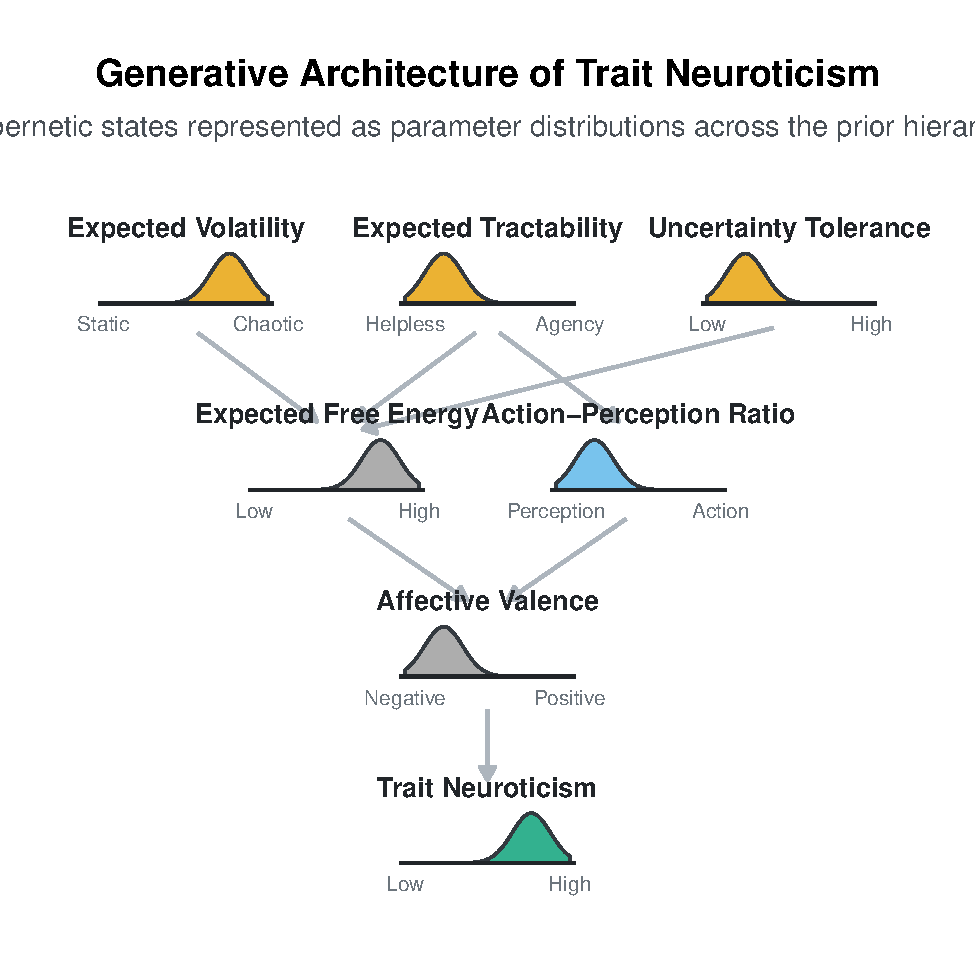
\includegraphics[keepaspectratio]{paper_files/figure-pdf/fig-cascade-1.pdf}}

\end{figure*}

\section{Hypothesized Factor
Structure}\label{hypothesized-factor-structure}

The fifteen dimensions of the CPC Model are not hypothesised to be
orthogonal. Rather, the cascade architecture implies systematic patterns
of co-variation. Characteristic configurations at higher levels
constrain, and therefore predict, characteristic configurations across
the lower-level dimensions. Five latent factors are hypothesised, each
representing a theoretically coherent syndrome of co-varying dimensions
expected to load together on factor-analytic assessment. These factors
are summarised in Table~\ref{tbl-factors}.

\begin{twocolumntable}

\begin{longtable}[]{@{}
  >{\raggedright\arraybackslash}p{(\linewidth - 4\tabcolsep) * \real{0.1235}}
  >{\raggedright\arraybackslash}p{(\linewidth - 4\tabcolsep) * \real{0.2112}}
  >{\raggedright\arraybackslash}p{(\linewidth - 4\tabcolsep) * \real{0.6653}}@{}}

\caption{\label{tbl-factors}Hypothesised five-factor structure of the
Core Priors Cascade Model. Each factor represents a theoretically
coherent syndrome of co-varying expectation and bias dimensions.}

\tabularnewline

\toprule\noalign{}
\begin{minipage}[b]{\linewidth}\raggedright
Factor
\end{minipage} & \begin{minipage}[b]{\linewidth}\raggedright
Primary Construct
\end{minipage} & \begin{minipage}[b]{\linewidth}\raggedright
Correlated Dimensions
\end{minipage} \\
\midrule\noalign{}
\endhead
\bottomrule\noalign{}
\endlastfoot
Factor 1: Epistemic Plasticity & How the agent handles new information &
Sensory-heavy sensory-prior bias; high epistemic-gain expectation; high
somatic-semantic bias; high noise expectation \\
Factor 2: Cybernetic Stability & Baseline expectation of safety versus
threat & High tractability expectation; positive affective valence (low
baseline EFE expectation); low volatility expectation \\
Factor 3: Blanket Permeability & How the self relates to the group &
High coupling bias (dissolution pole); high mentalizing bias \\
Factor 4: Temporal Extension & The timescale of the agent's generative
model & Deep temporal-depth expectation; terminal expectation
(transcendence pole); high coupling bias (differentiation pole) \\
Factor 5: Self-Model Stability & Temporal integration and coherence of
the self-model & High self-coherence expectation; high tractability
expectation; deep temporal-depth expectation (negative correlates: low
noise expectation; active cessation-seeking) \\

\end{longtable}

\end{twocolumntable}

These five factors carry clear functional correspondences to existing
descriptive models. Epistemic Plasticity maps broadly onto Openness to
Experience; Cybernetic Stability maps onto the inverse of Neuroticism,
with the baseline EFE expectation as its phenomenological felt
correlate; Blanket Permeability maps onto the affiliative pole of
Agreeableness and related communion constructs; and Temporal Extension
maps onto Conscientiousness. Self-Model Stability constitutes a
theoretically novel factor not cleanly captured by any single Big Five
dimension, intersecting with both Neuroticism and Conscientiousness
while carrying distinct clinical implications. The CPC Model's claim is
not that these five factors replace the Big Five but that they identify
the generative expectation and precision architecture from which Big
Five phenotypes emerge as behavioural expressions.

\section{Relationship to Existing
Models}\label{relationship-to-existing-models}

The CPC Model is positioned as a generative complement to the primary
existing frameworks in personality science, rather than a competitor to
them. Its relationship to each is considered in turn.

\subsection{Big Five Personality
Theory}\label{big-five-personality-theory}

The Big Five traits (\citeproc{ref-goldberg1990alternative}{Goldberg,
1990}; \citeproc{ref-mccrae1992introduction}{McCrae \& John, 1992})
represent the most extensively validated descriptive taxonomy of
personality. The CPC Model proposes to explain the mechanisms generating
the variance those dimensions capture. As noted above, Epistemic
Plasticity corresponds broadly to Openness to Experience; Cybernetic
Stability to the inverse of Neuroticism, with the baseline EFE
expectation acting as the phenomenological felt correlate of the
tractability-expectation configuration; Blanket Permeability to
Agreeableness-related constructs; and Temporal Extension to
Conscientiousness.

Extraversion, however, does not map cleanly onto any single CPC
dimension. It likely emerges from an interaction of the tractability
expectation, which drives approach motivation, and the coupling bias
(dissolution pole), which motivates social engagement and affiliation.
This non-correspondence is itself a prediction of the model: if
Extraversion reflects a combination of location and precision parameters
rather than a single dimension, it should not map cleanly onto any one
CPC factor, and its distinctive cross-factor loading pattern follows
accordingly.

\subsection{Hierarchical Taxonomy of Psychopathology
(HiTOP)}\label{hierarchical-taxonomy-of-psychopathology-hitop}

The Hierarchical Taxonomy of Psychopathology (HiTOP,
\citeproc{ref-kotov2017hitop}{Kotov et al., 2017}) has advanced a
dimensional, structural model of mental illness that supersedes
traditional categorical diagnoses. The CPC Model shares HiTOP's
hierarchical architectural ethos and provides a generative mechanism for
its empirically derived spectra. Within the CPC framework, the broad
spectra of HiTOP, such as Internalizing and Externalizing, can be
conceptualised as the phenotypic output of specific hyperparameter
configurations.

For instance, the Internalizing spectrum aligns with the downstream
consequences of a low tractability expectation combined with high
expected volatility (producing chronic expected free energy), whereas
the Externalizing spectrum may reflect the combined outputs of a high
differentiation coupling bias and a prior-heavy sensory-prior bias. By
mapping HiTOP's descriptive hierarchies onto the CPC's generative
expectations and precision biases, psychopathology can be understood not
merely as statistical deviations, but as rigid, self-reinforcing
cybernetic attractors on the free energy landscape.

\subsection{BIS/BAS Theory}\label{bisbas-theory}

Gray's (\citeproc{ref-gray1982neuropsychology}{1982}) Behavioural
Inhibition and Activation Systems provide a neurobiological account of
approach and avoidance motivation. The tractability expectation directly
formalises the BIS/BAS distinction within a generative modelling
framework. A high tractability expectation maps onto dominant BAS
functioning, characterised by sustained approach, reward sensitivity,
and behavioural activation. A low tractability expectation maps onto
dominant BIS functioning, characterised by behavioural inhibition,
hypervigilance to potential prediction errors, and an anxiety-prone
response to uncertainty.

The added theoretical value is mechanistic. BIS/BAS describes the
behavioural output; the CPC Model proposes the hierarchical expectation
structure that produces it, grounding the distinction in the mathematics
of expected free energy minimisation and extending it with the upstream
existential-level parameters (volatility expectation, noise expectation)
that modulate BIS/BAS expression.

\subsection{Attachment Theory}\label{attachment-theory}

The coupling bias and its associated boundary-level dimensions map
directly onto the attachment styles identified by Bowlby
(\citeproc{ref-bowlby1969attachment}{1969}) and Ainsworth. Avoidant
attachment corresponds to a coupling bias heavily skewed toward the
differentiation pole, combined with a low mentalizing bias. The agent
minimises expected free energy by maintaining rigid blanket boundaries
and discounting social prediction errors. Anxious-preoccupied attachment
corresponds to a coupling bias skewed toward the dissolution pole,
combined with a high mentalizing bias and a low tractability
expectation. The agent urgently seeks high coupling with attachment
figures but cannot trust the tractability of that coupling to resolve
relational uncertainty. Secure attachment corresponds to a calibrated,
flexible coupling bias and a high tractability expectation. The agent
can engage in adaptive coupling because it expects the resulting
prediction errors will be resolvable. The CPC formulation offers a
mechanistic account of why insecure attachment styles persist: they are
self-consistent configurations of interacting expectations and precision
allocations that are self-reinforcing across development.

\subsection{Sensation Seeking}\label{sensation-seeking}

Zuckerman's (\citeproc{ref-zuckerman1994behavioral}{1994})
sensation-seeking construct overlaps directly with the epistemic
foraging architecture. The novel contribution of the CPC framework is
splitting this drive into a generalized epistemic-gain expectation and a
domain-specific somatic-semantic bias. Existing sensation-seeking scales
conflate physical risk-taking with intellectual novelty-seeking within a
single dimension. The CPC Model hypothesises these to be partially
separable, predicting that the somatic and semantic foraging expressions
will show discriminant validity based on an individual's underlying
precision ratio. This hypothesis constitutes a direct, testable
empirical contribution requiring dedicated scale development and
factor-analytic verification.

\subsection{Cybernetic Big Five
Theory}\label{cybernetic-big-five-theory}

DeYoung's (\citeproc{ref-deyoung2015cybernetic}{2015}) Cybernetic Big
Five Theory (CB5T) represents the most direct theoretical antecedent of
the CPC Model. CB5T conceptualises the Big Five in cybernetic terms,
organising traits around two meta-traits, Plasticity and Stability,
grounded in generic reward and threat parameters. The CPC Model builds
on this framework by operationalising the underlying parameters within
the formal mathematics of the FEP.

Where CB5T describes an organism that ``reacts to threat,'' the CPC
Model specifies that the organism experiences an elevated baseline EFE
expectation arising from a low tractability expectation within a
high-volatility environment. DeYoung's Plasticity meta-trait corresponds
to the behavioural output of CPC Factor 1, and his Stability meta-trait
to CPC Factor 2. The CPC Model thus offers CB5T a formal mathematical
grounding, extending it with dimensions that lie outside CB5T's current
scope: the terminal expectation, the sensory-anchoring bias, and the
explicit somatic/semantic precision split.

\subsection{Jungian Archetypes}\label{jungian-archetypes}

Jungian archetypes can be formalised within the CPC framework as deeply
entrenched, phylogenetically conserved structural expectations
(\citeproc{ref-jung1968archetypes}{Jung, 1968}). Rather than literal
inherited images, evolutionary cognitive science reframes archetypes as
``core representations of social instincts'' designed to simulate and
predict recurrent ancestral challenges, such as self-protection, mating,
and social exchange (\citeproc{ref-becker2019archetypes}{D. V. Becker \&
Neuberg, 2019}).

Within the free energy landscape, these evolved social instincts
function as ``strange attractors''
(\citeproc{ref-becker2019archetypes}{D. V. Becker \& Neuberg, 2019}).
They represent ``shared minima'' or ``eigenmodes'' of the deep
unconscious, canalized across human phylogeny
(\citeproc{ref-mcgovern2025eigenmodes}{McGovern et al., 2025}). Drawing
on a trilogical interplay across the functional hierarchy, the
archetype's ``affective core'' originates in subcortical systems, gains
sensory manifestation (the ``archetypal image'') in lower-level
cortices, and ultimately achieves narrative form (the ``archetypal
story'') in high-level transmodal regions like the Default Mode Network
(\citeproc{ref-mcgovern2025eigenmodes}{McGovern et al., 2025}).

Under normal waking conditions, these global parameters operate in the
background to constrain proximal inference. However, during episodes of
extreme semantic foraging---when the agent deliberately weights
prediction errors heavily---superficial generative models collapse. As
the system falls back on these deeper phylogenetic attractors to prevent
catastrophic free energy increase, the agent consciously encounters the
bedrock of the human generative model: the ancient, affective structural
constraints inherited from our collective evolutionary past
(\citeproc{ref-mcgovern2025eigenmodes}{McGovern et al., 2025}).

\subsection{REBUS Model and Psychedelic
Research}\label{rebus-model-and-psychedelic-research}

The REBUS (Relaxed Beliefs Under Psychedelics) model
(\citeproc{ref-carhart2019rebus}{Carhart-Harris \& Friston, 2019})
provides a pharmacologically grounded account of how the expectation and
bias structure proposed by the CPC Model can be temporarily altered.
REBUS proposes that classical serotonergic psychedelics act via the
5-HT2A receptor to reduce the gain on descending prediction signals from
high-level cortical areas.

Within the CPC architecture, this equates to flattening the free energy
landscape. The typical top-down constraining influence of the higher
cortex is relinquished, permitting a more anarchic, bottom-up
information flow (\citeproc{ref-mcgovern2025eigenmodes}{McGovern et al.,
2025}). This flattening allows the deeply canalized, affect-laden
``archetypes as such'' residing in subcortical structures to propagate
upward and manifest consciously as vivid archetypal imagery
(\citeproc{ref-mcgovern2025eigenmodes}{McGovern et al., 2025}).

The therapeutic benefits reported in psychedelic-assisted treatment may
thus be understood as the functional consequence of transient
attractor-wall shallowing. The agent is temporarily liberated from
deeply entrenched, pathologically stable configurations and afforded the
opportunity to settle into adjacent basins with lower expected free
energy. The CPC Model generates specific predictions here: individuals
with highly entrenched precision walls (e.g., exceptionally high
Cybernetic Stability) may require greater perturbation to achieve
reorganisation, whereas those with shallower prior landscapes (e.g.,
high Epistemic Plasticity, low self-coherence expectations) may be
highly susceptible to destabilisation.

\section{Limitations and Open
Questions}\label{limitations-and-open-questions}

The Core Priors Cascade Model offers several contributions to the
theoretical landscape of personality science. First, by grounding
individual differences in the mathematics of the Free Energy Principle,
it provides a principled mechanistic account of why personality
configurations are stable, why they co-vary in the patterns observed by
descriptive models, and why certain configurations confer differential
psychopathological vulnerability. The cascade architecture implies that
interventions targeting operational-level parameters (as in most
cognitive and behavioural therapies) will have limited durability unless
existential and boundary-level expectations are also addressed, since
deep stability and chronic suffering are maintained by the structural
configuration at the highest levels of the hierarchy, not merely by
surface-level epistemic strategies.

Second, splitting the epistemic foraging drive into a generalized
epistemic-gain expectation and a domain-specific somatic-semantic bias
constitutes a theoretically motivated prediction not generated by
existing models. If confirmed by discriminant validity evidence, this
distinction would have implications for understanding heterogeneity
within sensation-seeking, risk tolerance, and creative openness.

Third, the terminal expectation provides a formal active inference
account of temporal self-extension and its pathological extremes. The
active cessation-seeking pole of the disengagement configuration, in
particular, offers a mechanistic reframing of suicidal ideation as a
specific, highly precise terminal expectation. Rather than treating it
as merely a symptom category, it conceptualizes ideation as the agent's
rational minimisation of expected free energy given an internal
architecture that renders all available future states unresolvably
costly.

Despite these contributions, several limitations and open questions
remain. The most pressing empirical challenge is developing valid
measurement instruments capable of assessing the proposed expectation
and bias parameters. Traditional subjective questionnaires predominantly
capture the ``observables'' of personality. They do not directly access
the unconscious expectations and precision weightings that form the
actual scaffolding of the human conscious experience. Because these
deeply entrenched generative parameters operate outside introspective
awareness, self-reports merely capture their downstream phenomenological
output.

However, this measurement gap is not insurmountable. By reliably
measuring these observables and rigorously analysing their covariance,
researchers can make robust inferences about the higher-order structural
expectations generating them. The latent variables modeled from dense,
high-quality psychometric data can serve as proxies for the deeper prior
landscape.

Furthermore, implicit behavioural tasks offer a promising alternative to
self-report. Because explicit questionnaires are vulnerable to
introspective limits, tasks that probe inference processes directly may
be better suited for assessing CPC dimensions. As demonstrated by
Makowski
(\citeproc{ref-makowski2023illusion}{\textbf{makowski2023illusion?}}),
who found systematic links between personality traits and illusion
sensitivity in a perceptual decision task, implicit measures can bypass
declarative awareness to probe the underlying predictive architecture
directly. A battery of perceptual, somatic, and cognitive tasks could
eventually serve as direct assays of the CPC Model's latent dimensions.
Computational psychiatry provides relevant methodological precedents
here (\citeproc{ref-huys2016computational}{Huys et al., 2016}), where
parameters analogous to the CPC's operational-level dimensions (learning
rates, sensory weightings, temporal discounting) have been successfully
back-estimated from task performance using hierarchical Bayesian models.

The CPC framework extends this tradition by situating these parameters
within an explicit expectation-bias hierarchy, generating the prediction
that different computational task designs will probe different levels.
Paradigms involving estimation of environmental volatility will tax
existential-level expectations; tasks involving social inference and
boundary detection will probe boundary-level biases; and tasks requiring
rapid strategy-switching under conflicting evidence will ngage
operational-level biases. Paradoxically, the most informative category,
existential-level expectations, will be the hardest to access directly.
Their influence operates precisely by suppressing the prediction errors
that would otherwise reveal them. Paradigms that systematically
manipulate volatility, tractability, and uncertainty across extended
task sequences may be best positioned to back-out these deep structural
parameters.

Additionally, the proposed five-factor structure is hypothetical and
awaits empirical validation. Factor-analytic assessment will be
necessary to determine the actual latent structure of co-variation
across CPC dimensions, and it is plausible that the factor structure
will vary across populations and developmental periods. Future work
should prioritise the development of psychometric and computational
modelling paradigms for parameter estimation, and longitudinal
investigation of how expectation and bias structures evolve across
development and in response to therapeutic intervention.

\section{References}\label{references}

\phantomsection\label{refs}
\begin{CSLReferences}{1}{0}
\bibitem[\citeproctext]{ref-bakan1966duality}
Bakan, D. (1966). \emph{The duality of human existence: An essay on
psychology and religion}. Rand McNally.

\bibitem[\citeproctext]{ref-barrett2017tce}
Barrett, L. F. (2017). The theory of constructed emotion: An active
inference account of interoception and categorization. \emph{Social
Cognitive and Affective Neuroscience}, \emph{12}(1), 1--23.

\bibitem[\citeproctext]{ref-becker2019archetypes}
Becker, D. V., \& Neuberg, S. L. (2019). Archetypes reconsidered as
emergent outcomes of cognitive complexity and evolved motivational
systems. \emph{Psychological Inquiry}, \emph{30}(2), 59--75.

\bibitem[\citeproctext]{ref-becker1973denial}
Becker, E. (1973). \emph{The denial of death}. Simon; Schuster.

\bibitem[\citeproctext]{ref-bowlby1969attachment}
Bowlby, J. (1969). \emph{Attachment and loss: Vol. 1. attachment}. Basic
Books.

\bibitem[\citeproctext]{ref-carhart2019rebus}
Carhart-Harris, R., \& Friston, K. J. (2019). {REBUS} and the anarchic
brain: Toward a unified model of the brain action of psychedelics.
\emph{Pharmacological Reviews}, \emph{71}(3), 316--344.

\bibitem[\citeproctext]{ref-craig2002feel}
Craig, A. D. (2002). How do you feel? Interoception: The sense of the
physiological condition of the body. \emph{Nature Reviews Neuroscience},
\emph{3}(8), 655--666.

\bibitem[\citeproctext]{ref-deyoung2015cybernetic}
DeYoung, C. G. (2015). Cybernetic big five theory. \emph{Journal of
Research in Personality}, \emph{56}, 33--58.

\bibitem[\citeproctext]{ref-erikson1968identity}
Erikson, E. H. (1968). \emph{Identity: Youth and crisis}. W. W. Norton
\& Company.

\bibitem[\citeproctext]{ref-eysenck1967biological}
Eysenck, H. J. (1967). \emph{The biological basis of personality}.
Charles C Thomas Publisher.

\bibitem[\citeproctext]{ref-fleeson2015whole}
Fleeson, W., \& Jayawickreme, E. (2015). Whole trait theory.
\emph{Journal of Research in Personality}, \emph{56}, 82--92.

\bibitem[\citeproctext]{ref-friston2010free}
Friston, K. (2010). The free-energy principle: A unified brain theory?
\emph{Nature Reviews Neuroscience}, \emph{11}(2), 127--138.

\bibitem[\citeproctext]{ref-friston2019markov}
Friston, K. (2019). A free energy principle for a particular physics.
\emph{arXiv Preprint arXiv:1909.10863}.

\bibitem[\citeproctext]{ref-gallagher2000philosophical}
Gallagher, S. (2000). Philosophical conceptions of the self:
Implications for cognitive science. \emph{Trends in Cognitive Sciences},
\emph{4}(1), 14--21.

\bibitem[\citeproctext]{ref-goldberg1990alternative}
Goldberg, L. R. (1990). An alternative "description of personality": The
big-five factor structure. \emph{Journal of Personality and Social
Psychology}, \emph{59}(6), 1216--1229.

\bibitem[\citeproctext]{ref-gray1982neuropsychology}
Gray, J. A. (1982). \emph{The neuropsychology of anxiety: An enquiry
into the functions of the septo-hippocampal system}. Clarendon Press.

\bibitem[\citeproctext]{ref-greenberg1986terror}
Greenberg, J., Pyszczynski, T., \& Solomon, S. (1986). The causes and
consequences of a need for self-esteem: A terror management theory.
\emph{Public Knowledge, Private Ignorance: Toward a Resolution of
Cognitive Dissonance}, 189--212.

\bibitem[\citeproctext]{ref-huys2016computational}
Huys, Q. J. M., Maia, T. V., \& Frank, M. J. (2016). Computational
psychiatry as a bridge from neuroscience to clinical applications.
\emph{Nature Neuroscience}, \emph{19}(3), 404--413.

\bibitem[\citeproctext]{ref-jung1968archetypes}
Jung, C. G. (1968). \emph{The archetypes and the collective
unconscious}. Princeton University Press.

\bibitem[\citeproctext]{ref-kotov2017hitop}
Kotov, R., Krueger, R. F., Watson, D., Achenbach, T. M., Althoff, R. R.,
Bagby, R. M., Brown, T. A., Carpenter, W. T., Caspi, A., Clark, L. A.,
et al. (2017). The hierarchical taxonomy of psychopathology (HiTOP): A
dimensional alternative to traditional nosologies. \emph{Journal of
Abnormal Psychology}, \emph{126}(4), 454.

\bibitem[\citeproctext]{ref-marcia1966development}
Marcia, J. E. (1966). Development and validation of ego-identity status.
\emph{Journal of Personality and Social Psychology}, \emph{3}(5),
551--558.

\bibitem[\citeproctext]{ref-mcadams1996personality}
McAdams, D. P. (1996). Personality, modernity, and the storied self: A
contemporary framework for studying persons. \emph{Psychological
Inquiry}, \emph{7}(4), 295--321.

\bibitem[\citeproctext]{ref-mccrae1992introduction}
McCrae, R. R., \& John, O. P. (1992). An introduction to the five-factor
model and its applications. \emph{Journal of Personality}, \emph{60}(2),
175--215.

\bibitem[\citeproctext]{ref-mcgovern2025eigenmodes}
McGovern, H., Aqil, M., Atasoy, S., \& Carhart-Harris, R. (2025).
Eigenmodes of the deep unconscious: The neuropsychology of jungian
archetypes and psychedelic experience. \emph{Neuroscience of
Consciousness}, \emph{2025}(1), niaf039.

\bibitem[\citeproctext]{ref-mischel1995cognitive}
Mischel, W., \& Shoda, Y. (1995). A cognitive-affective system theory of
personality: Reconceptualizing situations, dispositions, dynamics, and
invariance in personality structure. \emph{Psychological Review},
\emph{102}(2), 246.

\bibitem[\citeproctext]{ref-seligman1972learned}
Seligman, M. E. P. (1972). Learned helplessness. \emph{Annual Review of
Medicine}, \emph{23}(1), 407--412.

\bibitem[\citeproctext]{ref-seth2013interoceptive}
Seth, A. K. (2013). Interoceptive inference, emotion, and the embodied
self. \emph{Trends in Cognitive Sciences}, \emph{17}(11), 565--573.

\bibitem[\citeproctext]{ref-zuckerman1994behavioral}
Zuckerman, M. (1994). \emph{Behavioral expressions and biosocial bases
of sensation seeking}. Cambridge University Press.

\end{CSLReferences}






\end{document}
